% \documentclass[handout]{beamer}
\documentclass{beamer}

\mode<presentation>
{
  \usetheme{ANLBlue}
  % \usefonttheme[onlymath]{serif}
  % \usetheme{Singapore}
  % \usetheme{Warsaw}
  % \usetheme{Malmoe}
  % \useinnertheme{circles}
  % \useoutertheme{infolines}
  % \useinnertheme{rounded}

  \setbeamercovered{transparent=20}
}

\usepackage[english]{babel}
\usepackage[latin1]{inputenc}
\usepackage{alltt,listings,multirow,ulem,siunitx}
\usepackage[absolute,overlay]{textpos}
\TPGrid{1}{1}
\usepackage{pdfpages}
\usepackage{ulem}
\usepackage{multimedia}
\usepackage{multicol}
\newcommand\hmmax{0}
\newcommand\bmmax{0}
\usepackage{bm}
\usepackage{comment}
\usepackage{subcaption}

% font definitions, try \usepackage{ae} instead of the following
% three lines if you don't like this look
\usepackage{mathptmx}
\usepackage[scaled=.90]{helvet}
% \usepackage{courier}
\usepackage[T1]{fontenc}
\usepackage{tikz}
\usetikzlibrary{decorations.pathreplacing}
\usetikzlibrary{shadows,arrows,shapes.misc,shapes.arrows,shapes.multipart,arrows,decorations.pathmorphing,backgrounds,positioning,fit,petri,calc,shadows,chains,matrix}

\newcommand\vvec{\bm v}
\newcommand\bvec{\bm b}
\newcommand\bxk{\bvec_0 \times \kappa_0 \cdot \nabla}
\newcommand\delp{\nabla_\perp}

% \usepackage{pgfpages}
% \pgfpagesuselayout{4 on 1}[a4paper,landscape,border shrink=5mm]

\usepackage{JedMacros}

\newcommand{\timeR}{t_{\mathrm{R}}}
\newcommand{\timeW}{t_{\mathrm{W}}}
\newcommand{\mglevel}{\ensuremath{\ell}}
\newcommand{\mglevelcp}{\ensuremath{\mglevel_{\mathrm{cp}}}}
\newcommand{\mglevelcoarse}{\ensuremath{\mglevel_{\mathrm{coarse}}}}
\newcommand{\mglevelfine}{\ensuremath{\mglevel_{\mathrm{fine}}}}

%solution and residual
\newcommand{\vx}{\ensuremath{x}}
\newcommand{\vc}{\ensuremath{\hat{x}}}
\newcommand{\vr}{\ensuremath{r}}
\newcommand{\vb}{\ensuremath{b}}

%operators
\newcommand{\vA}{\ensuremath{A}}
\newcommand{\vP}{\ensuremath{I_H^h}}
\newcommand{\vS}{\ensuremath{S}}
\newcommand{\vR}{\ensuremath{I_h^H}}
\newcommand{\vI}{\ensuremath{\hat I_h^H}}
\newcommand{\vV}{\ensuremath{\mathbf{V}}}
\newcommand{\vF}{\ensuremath{F}}
\newcommand{\vtau}{\ensuremath{\mathbf{\tau}}}


\title{Software design and packaging for extensibility, provenance, and sharing}
\author{{\bf Jed Brown} \texttt{jedbrown@mcs.anl.gov}}

\begin{comment}
  There is more to developing successful scientific software than the
  core numerical implementation.  Slapping an open source license on the
  code does not mean an army of talented developers will swoop in and
  turn your work into a wonderful package that everyone loves.  This
  talk will discuss techniques to improve extensibility so that users
  and developers can extend your software to solve problems you never
  imagined; provenance so that published results can be understood,
  reproduced, and extended; and facilitate sharing of enhancements,
  configurations, and benchmarks to advance the software capability and
  encourage a vibrant and insightful community
\end{comment}

% - Use the \inst command only if there are several affiliations.
% - Keep it simple, no one is interested in your street address.
% \institute
% {
%   Mathematics and Computer Science Division \\ Argonne National Laboratory
% }

\date{CIG Webinar, 2014-11-13 \\[1em]
This talk: \url{http://59A2.org/files/20141113-Software.pdf}}

% This is only inserted into the PDF information catalog. Can be left
% out.
\subject{Talks}


% If you have a file called "university-logo-filename.xxx", where xxx
% is a graphic format that can be processed by latex or pdflatex,
% resp., then you can add a logo as follows:

% \pgfdeclareimage[height=0.5cm]{university-logo}{university-logo-filename}
% \logo{\pgfuseimage{university-logo}}



% Delete this, if you do not want the table of contents to pop up at
% the beginning of each subsection:
% \AtBeginSubsection[]
% {
% \begin{frame}<beamer>
%   \frametitle{Outline}
%   \tableofcontents[currentsection,currentsubsection]
% \end{frame}
% }

% \AtBeginSection[]
% {
%   \begin{frame}<beamer>
%     \frametitle{Outline}
%     \tableofcontents[currentsection]
%   \end{frame}
% }

% If you wish to uncover everything in a step-wise fashion, uncomment
% the following command:

% \beamerdefaultoverlayspecification{<+->}

\begin{document}
\lstset{language=C}
\normalem

\begin{frame}
  \titlepage
\end{frame}

\begin{frame}{Firetran!}
  \begin{itemize}
  \item Renders HTML 10\% faster than Firefox or Chromium.
  \item<2-> but only if there is no JavaScript
    \begin{itemize}
    \item recompile to use JavaScript
    \end{itemize}
  \item<3-> Character encoding compiled in
  \item<4-> Mutually incompatible forks
  \item<5-> No confusing run-time proxy dialogs, edit file and recompile
  \item<5-> Proxy configuration compiled in
  \item<6-> For security, HTTP and HTTPS mutually incompatible
  \item<7-> Address in configuration file, run executable to render page
  \item<8-> Tcl script manages configuration file
  \item<9-> Plan to extend script to recompile Firetran with optimal features for each page.
  \end{itemize}
\end{frame}

\begin{frame}{Firetran struggles with market share}
  \begin{itemize}
  \item Status quo in many scientific software packages
  \item Why do we tolerate it?
  \item Is scientific software somehow different?
  \end{itemize}
\end{frame}

\begin{frame}{Trends in Computational Science}
  \begin{itemize}
  \item multiphysics, multiscale
  \item data assimilation, inversion, UQ
  \item risk-aware design and decision
  \item deeper software stacks
  \item many forms of extensibility
  \item artificial bottlenecks
  \end{itemize}
\end{frame}

\begin{frame}{Compile-time configuration}
  \begin{itemize}
  \item configuration in build system
  \item over-emphasis on ``efficiency''
  \item templates are compile-time
    \begin{itemize}
    \item combinatorial number of variants
    \end{itemize}
  \item compromises on-line analysis capability
  \item create artificial IO bottlenecks
  \item offloads complexity to scripts and ``workflow'' tools
  \item limits automation and testing of calibration
  \item maintaining consistency complicates provenance
  \end{itemize}
\end{frame}

\begin{frame}{Model coupling}
  \begin{itemize}
  \item Hero codes
    \begin{itemize}
    \item visionary scientist in single domain
    \item each package is king of its own environment
    \end{itemize}
  \item holes in knowledge exist at gaps between existing models
  \item models operate at different scales with different uncertainties
  \item coupling is hard enough with well-behaved components
  \item think like a library developer
    \begin{itemize}
    \item minimize assumptions about environment
    \item no globals, act locally, be explicit
    \item successes: compilers, web browsers, databases
    \end{itemize}
  \end{itemize}
\end{frame}

\begin{frame}{Provenance and Usability}
  \begin{itemize}
  \item How to capture all configuration knobs so experiment can be reproduced?  Compare
    \begin{itemize}
    \item single run-time configuration file
    \item compile-time configuration, multiple build systems, files passed between stages
    \end{itemize}
  \item transitive dependencies must also be good libraries
  \item plugins better than source modification
  \end{itemize}
\end{frame}

\begin{frame}{``Big'' Data}
  \begin{itemize}
  \item Workflows with multiple executables pass data through file system
  \item About 1 hour to read/write contents of volatile memory
  \item Global storage as \emph{alogrithmic} mechanism is dead
    \begin{itemize}
    \item Better to run in-core on a larger machine
    \item Out-of-core on full machine blows annual compute budget in one shot
    \end{itemize}
  \item Circumvent IO bottleneck by passing data in-memory to next stage
  \end{itemize}
\end{frame}

\begin{frame}{Nested dependencies}
  \begin{itemize}
  \item Encapsulation is important to control complexity
  \item Reconfiguring indirect dependencies breaks encapsulation
  \item Single library may be used by multiple components in executable
    \begin{itemize}
    \item diamond dependency graph
    \item conflict unless same version/configuration can be used for both
    \end{itemize}
  \end{itemize}
\end{frame}

\begin{frame}{Packaging and distribution}
  \begin{itemize}
  \item Developers underestimate challenge of installing software
  \item User experience damaged even when user's fault (broken environment)
  \item Package managers (Debian APT, RedHat RPM, MacPorts, Homebrew, etc.)
  \item Binary interface stability critical to packagers
  \end{itemize}
\end{frame}

\begin{frame}{User modifications versus plugins}
  \begin{itemize}
  \item Fragmentation is expensive and should be avoided
  \item Maintaining local modifications causes divergence
  \item Better to contain changes to a plugin
  \item \texttt{dlopen()} and register implementations in the shared library
  \item Invert dependencies and avoid loops
    \begin{itemize}
    \item \texttt{libB} depends on \texttt{libA}
    \item want optional implementation of \texttt{libA} that uses \texttt{libB}
    \item \texttt{libA-plugin} depends on both \texttt{libA} and \texttt{libB}
    \end{itemize}
  \item Static libraries are anti-productive (tell your computing center)
    \begin{itemize}
    \item Can sort-of do plugins by changing link line
    \end{itemize}
  \end{itemize}
\end{frame}

\begin{frame}{Controlling transitive complexity}
  \begin{itemize}
  \item Implementation complexity must not leak into public interface
  \item Choose good defaults and provide a way to configure inner parts
  \item Inversion of Control (``dependency injection'', ``service locator'')
  \item Can be multiple instances of components; identify using ``prefix'' rule
  \item Some use embedded Turing-complete configuration/scripting language
  \end{itemize}
\end{frame}

\begin{frame}{Object-oriented design}
  \begin{itemize}
  \item Should all errors be compile-time errors?
  \item Sounds good in theory, but brittle
    \begin{itemize}
    \item Should matrices have computable entries?
    \item Should the diagonal be extractable?
    \item Can the transpose be applied?
    \item Do ``Neumann'' subproblems exist?
    \item Different preconditioners require different properties from \texttt{Matrix}
    \end{itemize}
  \end{itemize}
\end{frame}

\begin{frame}{Controlling the Binary interface}
  \begin{itemize}
  \item Recompiling code is wasted productivity
  \item Implementation concerns (private variables, new virtual methods) should not require recompiling user code
  \item PETSc uses opaque pointers and the ``delegator'' (aka. ``pointer to implementation'') pattern.
  \item Static function overhead insignificant, incremental cost less than 2 cycles
  \item Better for debugging
  \item Easier to expose libraries to dynamic programming languages
  \end{itemize}
\end{frame}

\begin{frame}{Just-in-Time Compilation (JIT)}
  \begin{itemize}
  \item Fine-grained composition benefits from inlining
  \item Dynamic dispatch a much better library interface
  \item Templating not extensible via plugins, bloated, slow to compile
  \item JIT is promising for dynamic kernel fusion, plugin-style packaging
  \end{itemize}
\end{frame}

\begin{frame}{Upstreaming and community building}
  \begin{itemize}
  \item Maintainers should provide good alternatives to forking
  \item Welcoming environment for contributions
  \item Privacy, ``scooping'', openness
    \begin{itemize}
    \item My opinion: social problem, deal with using social means
    \end{itemize}
  \item Major tech companies have grossly underestimated cost of forking
  \item In science, we cannot pay off technical debt incurred by forking
  \item Provide extension points to reduce cost of new development
  \end{itemize}
\end{frame}

\section{Development Workflow}
\begin{frame}{Workflow ideals}
  \begin{itemize}
  \item 'master' is always stable and ready to release
  \item features are complete and tested before appearing in 'master'
  \item commits are minimal logically coherent, reviewable, and testable units
  \item related commits go together so as to be reviewable and debuggable by specialist
  \item new development is not disrupted by others' features and bugs
  \item rapid collaboration between developers possible
  \item \texttt{git log -{}-first-parent maint..master} reads like a changelog
  \item bugs can be fixed once and anyone that needs the fix can obtain it without side-effects
  \end{itemize}
\end{frame}

\begin{frame}{Simplified gitworkflows(7)}
  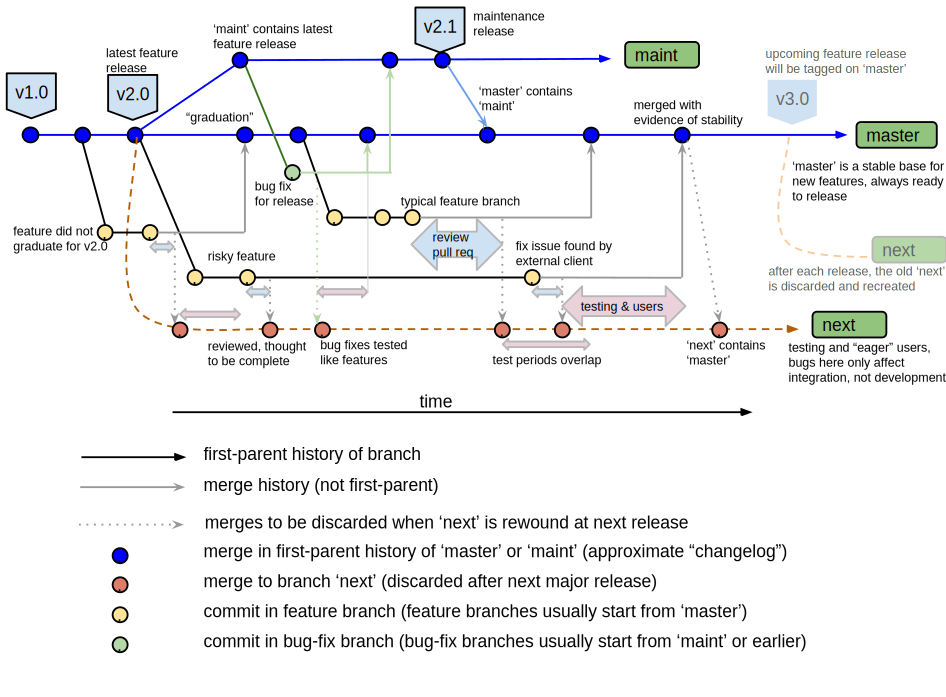
\includegraphics[width=\textwidth]{figures/Git/simplified-gitworkflows7.pdf}
\end{frame}

\begin{frame}{Best practices}
  \begin{itemize}
  \item Every branch has a purpose
  \item Distinguish integration branches from topic branches
  \item Do all development in topic branches
    \begin{itemize}
    \item \texttt{git checkout -b my/feature-branch master}
    \end{itemize}
  \item Namespace your branches if working on a shared repository
  \item Merge integration branches ``forward''
    \begin{itemize}
    \item \texttt{maint-1} $\to$ \texttt{maint} $\to$ \texttt{master} $\to$ \texttt{next}
    \item \texttt{git checkout -b my/bugfix-branch maint-1}
    \end{itemize}
  \item Write clear commit messages for reviewers and people trying to debug your code
  \item \href{https://bitbucket.org/petsc/petsc/wiki/developer-instructions-git\#markdown-header-merging}{Avoid excessive merging from upstream}
    \begin{itemize}
    \item Always write a clear commit message explaining what is being merged and why
    \end{itemize}
  \item Always merge topic branches as non-fast-forward (\texttt{merge -{}-no-ff})
  \item \href{https://bitbucket.org/petsc/petsc/wiki/developer-instructions-git\#markdown-header-racy-integration}{Gracefully retry if you lose a race to shared integration branch}
    \begin{itemize}
    \item This maximizes utility of \texttt{-{}-first-parent} history
    \end{itemize}
  \end{itemize}
\end{frame}

\begin{frame}{Outlook}
  \begin{itemize}
  \item Think like a library developer
  \item Avoid assumptions about environment
  \item Make everything a run-time decision
  \item Control complexity
  \item Encourage contributions
  \item Plan for creative new directions you haven't thought of yet
  \end{itemize}
\end{frame}


\end{document}
